\section{Quantum Communication Complexity}

\subsection{Quantum Computing}
\begin{frame}{Qubits}
    \begin{figure}
        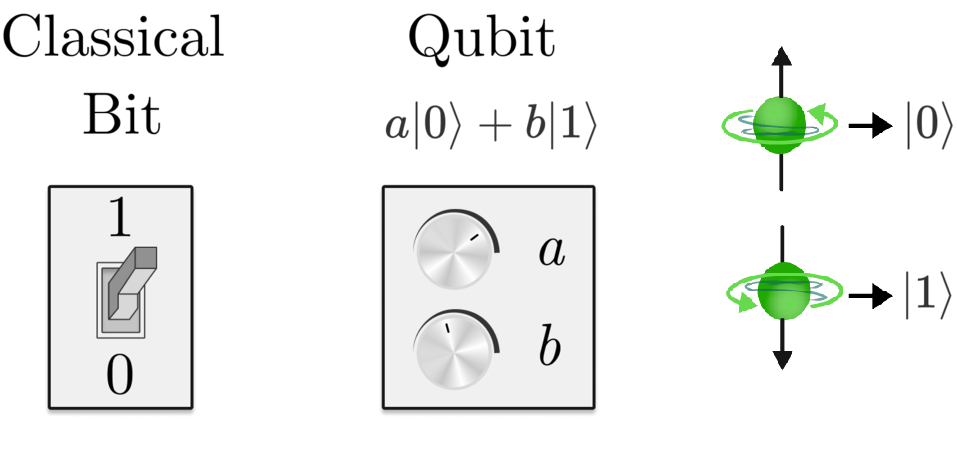
\includegraphics[width=.8\linewidth]{pics/y8XA7Re44P-frame-27.png}
        \label{fig:my_label}
    \end{figure}
    \begin{center}
    \begin{itemize}
        \uncover<+->{\item Prob $(state = |0\rangle) = a^2$}
        \uncover<+->{\item Prob $( state = |1\rangle) = b^2$}
        \uncover<+->{\item $a, b \in \mathbb{C}$}
    \end{itemize}
    \end{center}
\end{frame}

\begin{frame}{Deutsch-Jozsa Algorithm}
    \begin{figure}
        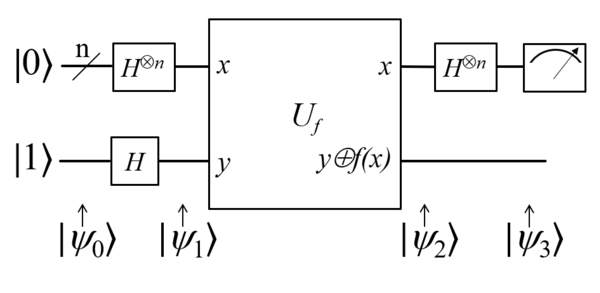
\includegraphics[width=.8\linewidth]{pics/600px-Deutsch-Jozsa-algorithm-quantum-circuit.png}
        \label{fig:my_label}
    \end{figure}
    \begin{center}
    \begin{itemize}
        \uncover<+->{\item Input: A binary function $f: \{0,1\}^n \rightarrow \{0,1\}$}
        \uncover<+->{\item Promised that function is either constant or balanced. }
        \uncover<+->{\item Output: Which?}
        \uncover<+->{\item Can be done in polytime with qc, but needs exponential time in a cc.}
    \end{itemize}
    \end{center}
\end{frame}
\begin{frame}{Grover's Algorithm}
    \begin{figure}
        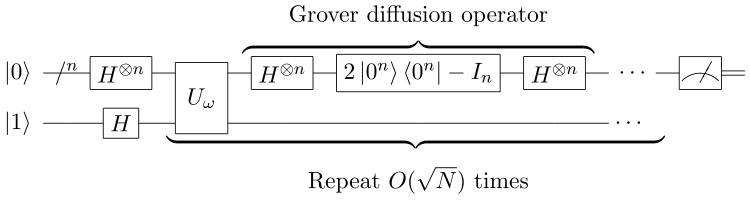
\includegraphics[width=\linewidth]{pics/750px-Grovers_algorithm.svg.png}
        \label{fig:my_label}
    \end{figure}
    \begin{center}
    \begin{itemize}
        \uncover<+->{\item Input: A function $f: \{0,1\}^n \rightarrow \{0,1\}^n$}
        
        \uncover<+->{\item Output: Find $x$, where $f(x) = y$.}
        \uncover<+->{\item Can be done in $O(\sqrt{n})$ with a quantum computer using Grover's Algorithm, but needs $O(n)$ time in the classical setting.}
    \end{itemize}
    \end{center}
\end{frame}
\subsection{Quantum Communication Complexity}
\begin{frame}{Can we do better?}
    \begin{center}
        
    \begin{itemize}
        \uncover<+->{\item We need $2^n - 1$ states to describe an $n$ qubit state}
        \uncover<+->{\item \textbf{Holevo's Theorem} says that with direct transmission, only $n$ bits can be communicated with $n$ qubits.}
        \uncover<+->{\item So, to no avail?}
    \end{itemize}\end{center}
\end{frame}

\begin{frame}{Equality}
    \begin{center}
        
    \begin{itemize}
        \uncover<+->{\item Distributed Deutsch-Jozsa}
        \uncover<+->{\item Promise version of Equality. Two inputs are either equal, or different at exactly half of the bits.}
        \uncover<+->{\item Has $O(\log n)$ CC, Classic is $O(n)$!}
    \end{itemize}\end{center}
\end{frame}

\begin{frame}{Disjointness}
    \begin{itemize}

        \uncover<+->{\item $z = x \wedge y, \quad z_i = x_i \wedge y_i$}
        \uncover<+->{\item $z_i$ is 1 iff $x_i = y_i$}
        \uncover<+->{\item Solving disjointness is finding $i$ where $z_i = 1$.}
                \uncover<+->{\item Distributed Grover's}
        \uncover<+->{\item Has $O( \log n \sqrt{n})$ CC, Classic is $O(n)$!}
    \end{itemize}
\end{frame}